\documentclass[12pt]{article}
\def\activityid{F07-K-v2}\usepackage[letterpaper,margin=.65in,top=.60in,bottom=.65in]{geometry}
\usepackage[T1]{fontenc}\usepackage[default]{sourcesanspro}
\usepackage{microtype,tikz,array,tabularx,fancyhdr,amsmath}\usepackage[hidelinks]{hyperref}
\usetikzlibrary{arrows.meta,calc}
\setlength{\parindent}{0pt}\setlength{\parskip}{7pt}\setlength{\headheight}{0pt}\setlength{\footskip}{26pt}\setlength{\emergencystretch}{2em}
\pagestyle{fancy}\fancyhf{}\renewcommand{\headrulewidth}{0pt}\renewcommand{\footrulewidth}{.4pt}
\fancyfoot[L]{\scriptsize Bellingham Math Circle / Week 7 / \activityid}\fancyfoot[R]{\scriptsize \thepage}
\definecolor{ink}{gray}{.12}\definecolor{soft}{gray}{.95}\color{ink}
\newcommand{\PageTitle}[2]{{\fontsize{10}{12}\selectfont\bfseries WEEK 7\quad GAME LAB\hfill #1\par}\vspace{3pt}{\fontsize{26}{29}\selectfont\bfseries #2\par}\vspace{2pt}}
\newcommand{\NameLine}{{\small Name: \rule{2.65in}{.4pt}\hfill Date: \rule{1.35in}{.4pt}\par}\vspace{4pt}}
\newcommand{\Task}[2]{\par\vspace{3pt}{\large\bfseries #1}\par #2\par}
\newcommand{\Subhead}[1]{\par\vspace{3pt}{\large\bfseries #1}\par}
\newcommand{\RuleBox}[1]{\par\begingroup\setlength{\fboxsep}{8pt}\colorbox{soft}{\parbox{\dimexpr\linewidth-16pt\relax}{#1}}\endgroup\par}
\newcommand{\WriteBox}[2]{\par\textbf{#1}\par\vspace{2pt}\begin{tikzpicture}\draw[black!40,line width=.5pt] (0,0) rectangle (\dimexpr\linewidth-.5pt\relax,#2);\end{tikzpicture}\par}
\newcommand{\StudentFooter}{\vfill{\small Build first. Explain by pointing, talking, or drawing.}\par}
\newcommand{\Code}[1]{\texttt{#1}}

\hypersetup{pdftitle={Week 7: k-1}}
\begin{document}
\PageTitle{K--1}{Can you leave a little trap?}\NameLine
\RuleBox{Two players alternate. Take \textbf{1 or 2} counters each turn. Never take more than remain. Taking the last counter wins.}\Task{1. Play first.}{Try piles of 4 and 5 counters. Trade the first turn. Check every move.}
\Task{2. A pile of three.}{Choose first or second. If you choose second, show what you will do after \textbf{either} of the first player's moves.}\begin{center}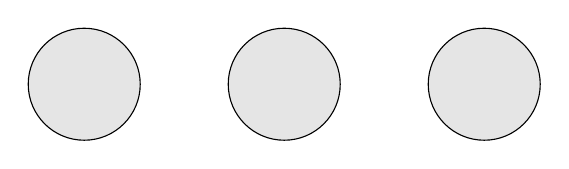
\begin{tikzpicture}[x=1in,y=1in]\foreach \x in {0,1,2}{\draw[fill=black!10](\x,0)circle(.28);}\end{tikzpicture}\end{center}
\WriteBox{If the first player takes 1, I will...}{1in}
\WriteBox{If the first player takes 2, I will...}{1in}
\Task{3. Tell the whole story.}{Does your plan work only when your partner helps, or against both choices? Demonstrate both branches with counters.}\StudentFooter
\newpage
\PageTitle{K--1}{A trap that grows}\NameLine
\RuleBox{Two players alternate. Take \textbf{1 or 2} counters each turn. Never take more than remain. Taking the last counter wins.}\Task{4. Try six counters.}{Arrange them as two groups of three. Can the second player answer every move and leave exactly three?}\begin{center}
\begin{tikzpicture}[x=.75in,y=.75in]\foreach \x in {0,1,2,4,5,6}{\draw[fill=black!10](\x,0)circle(.23);}\end{tikzpicture}\end{center}
\WriteBox{My two replies from six:}{1.05in}
\Task{5. Choose first or second.}{Try piles of 7, 8, and 9. Circle the piles you would like the \textbf{other player} to receive. Explain by playing.}
\begin{center}{\Huge 7\qquad8\qquad9}\end{center}
\WriteBox{What can I leave after the other player's turn and my reply?}{1.05in}
\textbf{Go further:} Could the same plan work with three groups of three? Four groups? You can prove it by describing how one whole group disappears in each pair of turns.\StudentFooter
\end{document}
